\documentclass[aps,prl,reprint]{revtex4-1}
\usepackage{blindtext}

\usepackage{amsmath}
\usepackage{graphicx}
\usepackage{commath}
\usepackage{siunitx}
\usepackage{tabularx}
\usepackage{subcaption}

\usepackage{amssymb}

\usepackage{float}

\usepackage{graphicx}


\usepackage[b]{esvect}


\newcommand{\de}{\mathrm{d}}
\newcommand{\vcc}{V_\text{CC}}
\newcommand{\parallelsum}{\mathbin{\!/\mkern-5mu/\!}}


\graphicspath{ {images/} }
\begin{document}

\title{Unit 7: Comparitors, Converters and Computers}
\author{Xueqi Li}
% \email{xueqi.li@stonybrook.edu}
\thanks{Partner: Tianming Hai}
\noaffiliation
\date{May 4, 2018}



% \begin{abstract}
% In this lab we introduced operational amplifier and the negative feedback. Furthermore, a few importent applications of amplifier, such as follower, inverting and non-inverting amplifier, integrator, and differentiator were discussed and their output voltage formulas have been derived. Moreover, the limit of the opamp was explored and two methods to measure the slew rate have been given as examples.
% \end{abstract}

\maketitle

\section{Introduction}
    One can translate a analog signal into digital signal, or trnaslate digital signal to analog. In here, we introduce the rule we want to translate the signal.
    \subsection{Translation Rule}
    In here we want to have a ``bijective'' function between agalog signal and digital. The set of the analog signal is just a interval of real number, let say $[V_i,V_f]$, and the set of the digital is a binary number with some fix length, let say $\mathbb{B}^n$, where $n$ is the length of the binary number string. 

    We see that it is not possible to have a real bijective function, since $|[V_i, V_f]| \neq |\mathbb{B}^n|$ but we can do that with some resolution, depend on $n$. The number can be represent for a $n$ length binary number is $2^n$, which is the resolution we can have. Thus, we can think analog signal is a set of interval as following:
    \[
    \{[V_i, V_i + \frac{\Delta V}{2^n}),[V_i + \frac{\Delta V}{2^n}, V_i + 2\frac{\Delta V}{2^n})\cdots [V_f - \frac{\Delta V}{2^n},V_f]\}
    \]
    where $\Delta V = V_f - V_i$, Let define $a_k:=[V_i + k \frac{\Delta V}{2^n}, V_i + (k+1)\frac{\Delta V}{2^n})$, Thus we have:
    \begin{align*}
        \mathbb{A} &= \{[V_i + k \frac{\Delta V}{2^n}, V_i + (k+1)\frac{\Delta V}{2^n}): k \le 2^n - 1\}\\
                   &= \{a_k:k\in \mathbb{Z},0 \le k \le 2^n - 1\}
    \end{align*}
    Now we see it is possible to define a bijective between $\mathbb{A}$ to $\mathbb{B}^n$ since $|\mathbb{A}| = 2^n = |\mathbb{B}^n|$. Thus, we can defined our fucntion as following:
    \begin{align*}
        \Lambda(a_k) &= \text{Bin}\lfloor k\rfloor ;\\
        \Lambda^{-1}(b) &= a_{\text{Dec}(b)}
    \end{align*}
    where $\text{Bin}: \mathbb{R} \rightarrow \mathbb{B}^n$ maps a real number's interger part to its binary string and its ``inverse'' function is $\text{Dec}: \mathbb{B}^n \rightarrow \mathbb{Z}$ maps the binary string to the number it represent.

    We can defined $\varsigma$ to be the function gives the infimum of $a_k\in\mathbb{A}$ as following:
    \begin{align*}
        \varsigma(a_k) &= \inf(a_k) = V_i + k \frac{\Delta V}{2^n};\\
        \varsigma^{-1}(V)&= a_{\lfloor(V-V_i)\frac{2^n}{\Delta V} \rfloor}
    \end{align*}

    Than the translation between analog and digital signal is juat the composition of $\varsigma$ and $\Lambda$:
    \begin{align}
        \Xi (V) &= \varsigma^{-1} \circ \Lambda (V) = \text{Bin}\lfloor (V-V_i)\frac{2^n}{\Delta V} \rfloor;\label{eq:anaToDig}\\
        \Xi^{-1} (b)&= \Lambda^{-1} \circ \varsigma(V) = V_i + \text{Dec}(b) \frac{\Delta V}{2^n} \label{eq:digToAna}
    \end{align}

    \subsubsection{Zero Minimum Voltage}
        Let say if we have $V_i = 0$, $V_f = V_\text{ref}$. We see that $\Delta V = V_\text{ref}$. Thus the Equation~\ref{eq:anaToDig} and Equation~\ref{eq:digToAna} reduced to
        \begin{align}
            \Xi_0 (V) &= \text{Bin}\lfloor V\frac{2^n}{V_\text{ref}} \rfloor; \label{eq:anaToDig.zero}\\ 
            \Xi^{-1}_0 (b)&= \text{Dec}(b) \frac{V_\text{ref}}{2^n} \label{eq:digToAna.zero}
        \end{align}
\section{Data and Calculation}
    In the lab we are using 8 bit ADC and DAC chip to translate digital and analog signal back and forth.
    \subsection{DAC}
        \begin{figure}[h]
            \centering
            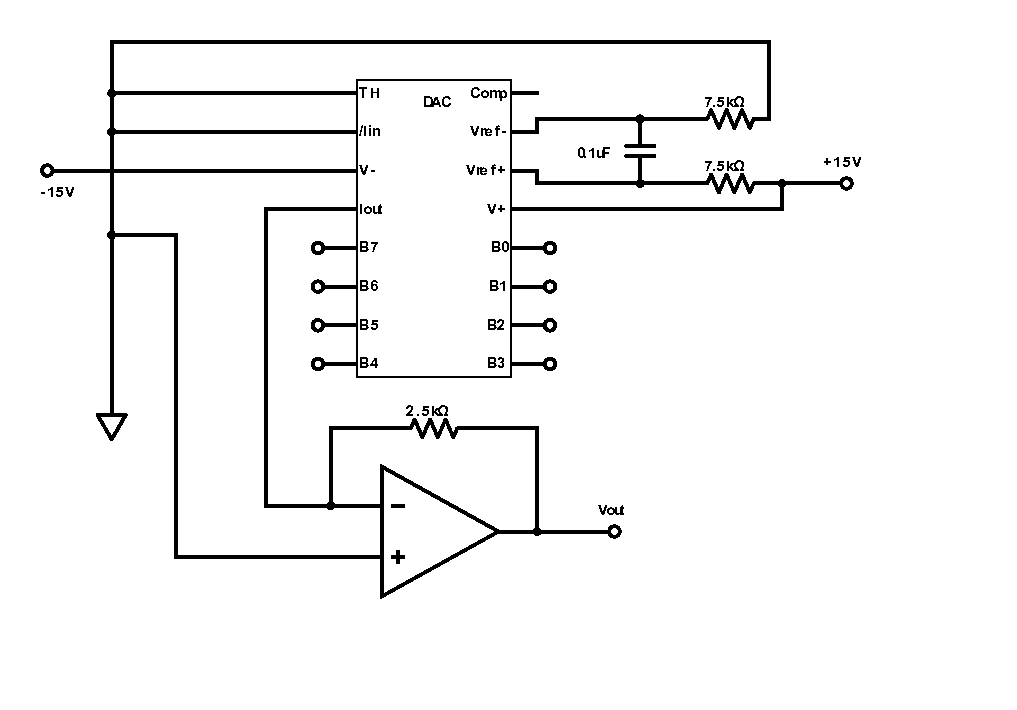
\includegraphics[width=0.49\textwidth]{image/DAC.pdf}
            \caption{DAC circuit in lab}
            \footnotetext{B0 to B7 are connect to development board}
            \label{fig:dac}
        \end{figure}
        In lab we use a circuit in Figure~\ref{fig:dac}. The reason we do so is because the DAC used in lab is output a current. Thus we need to use the opamp to convert current to voltage. 

        In here, we want to limit the current on around 4mA. $\vcc$ is given as 15V, so we found the resistor on DAC chip is around 7.5k$\Omega$. It follows that the resistor on opamp is $\frac{1}{3}$ of the resistor on DAC chip, which is 2.5k$\Omega$. In the lab we measure the resistor on DAC is 7.28(2)k$\Omega$ and the resistor on opamp is 2.3(1)k$\Omega$.

        \begin{table}[h]
            \begin{ruledtabular}
                \begin{tabular}{ccc}
                    Input Number & Output Voltage [V] & Error on Output [V] \\ \hline
                    0 & 0.12 & 0.02 \\
                    16 & 0.42 & 0.02 \\
                    32 & 0.74 & 0.02 \\
                    48 & 1.06 & 0.02 \\
                    64 & 1.38 & 0.02 \\
                    80 & 1.70 & 0.02 \\
                    96 & 2.00 & 0.02 \\
                    112 & 2.30 & 0.02 \\
                    128 & 2.64 & 0.02 \\
                    144 & 2.92 & 0.02 \\
                    160 & 3.24 & 0.02 \\
                    176 & 3.58 & 0.02 \\
                    192 & 3.90 & 0.02 \\
                    208 & 4.20 & 0.02 \\
                    224 & 4.54 & 0.02 \\
                    240 & 4.84 & 0.02 \\
                \end{tabular}
            \end{ruledtabular}
            \caption{Output of DAC}
            \footnotetext{Error is from minimum scale of scope.}
            \label{table:dac}
        \end{table} 
        \begin{figure}[h]
            \centering
            \includegraphics[width=0.49\textwidth]{image/plot.pdf}
            \caption{Linear fit of DAC data}
            \footnotetext{Some error bar may too small to see}
            \label{fig:dacPlot}
        \end{figure}

        In the lab, we measure the output voltage. The data obtained is in Table~\ref{table:dac}. After a linear fix, we find the slope is 0.020V with an error of $6.78\times 10^5$V and the offset is 0.111V with an error of $9.12\times 10^5$V, as present in Figure~\ref{fig:dacPlot}.
    \subsection{ADC}
        \begin{figure}[h]
            \centering
            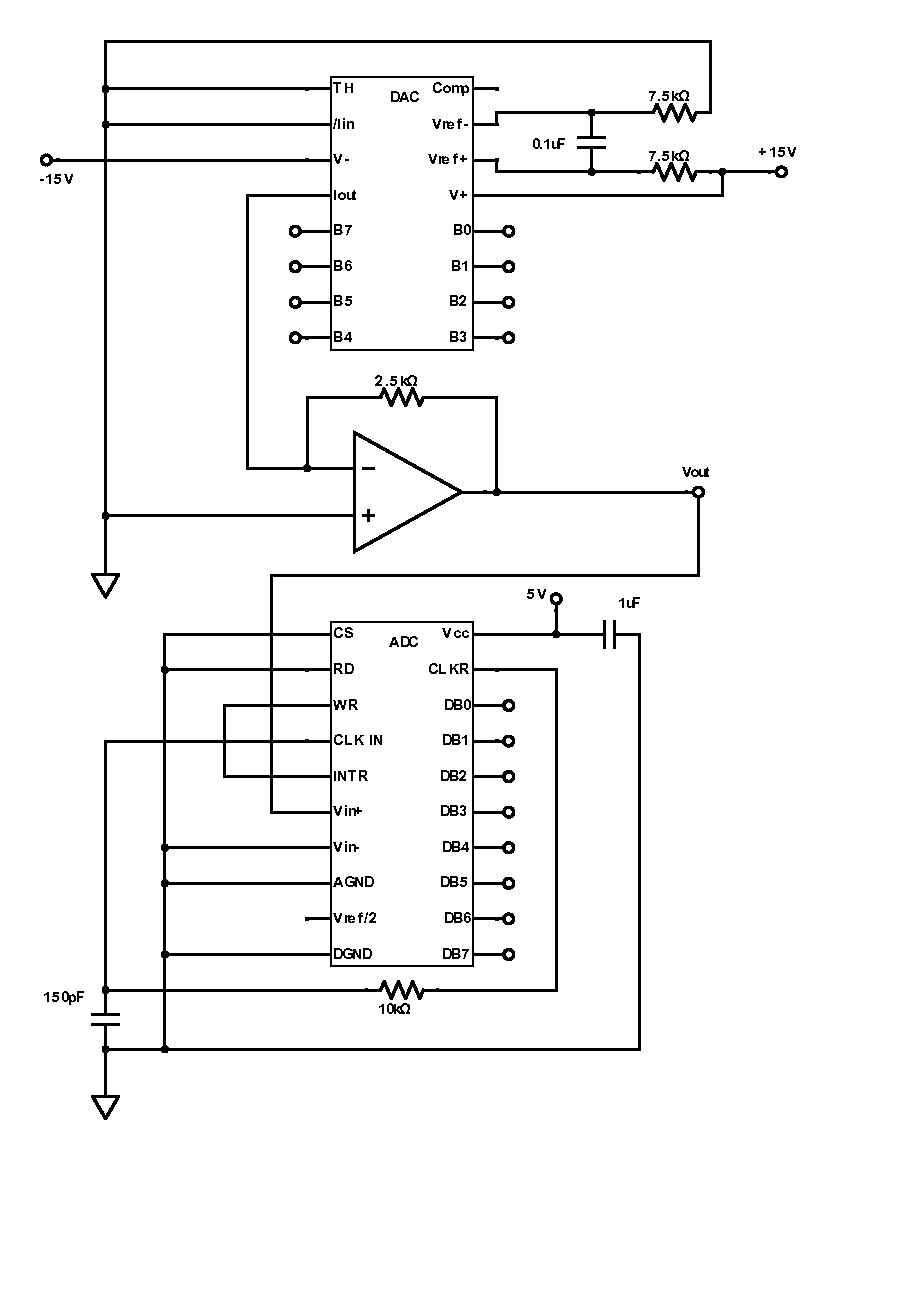
\includegraphics[width=0.49\textwidth]{image/DAC-ADC.pdf}
            \caption{Link the output of DAC to the input of ADC}
            \footnotetext{B0 to B7 are connect to development board}
            \footnotetext{DB0 to DB7 are connect to development board}
            \label{fig:adc}
        \end{figure}
        \begin{figure}[h]
            \centering
            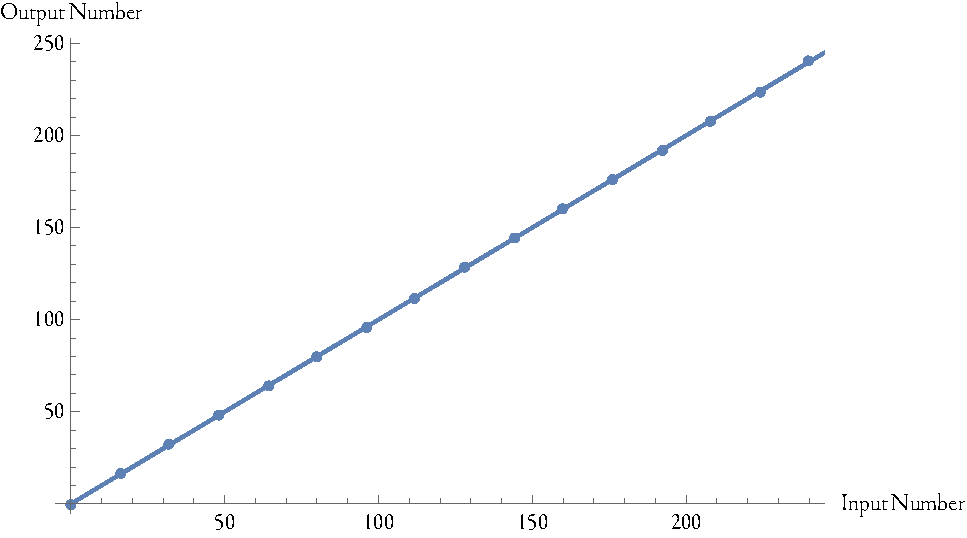
\includegraphics[width=0.49\textwidth]{image/plot2.pdf}
            \caption{result of DAC}
            \label{fig:adcPlot}
        \end{figure}
        In this part, connect the output of DAC to the input of ADC. In the lab we see that the input from the development board is same as the output to the development board for every input, as present in Figure~\ref{fig:adcPlot}.
    \subsection{Sine Wave}
        \begin{figure}[h]
            \centering
            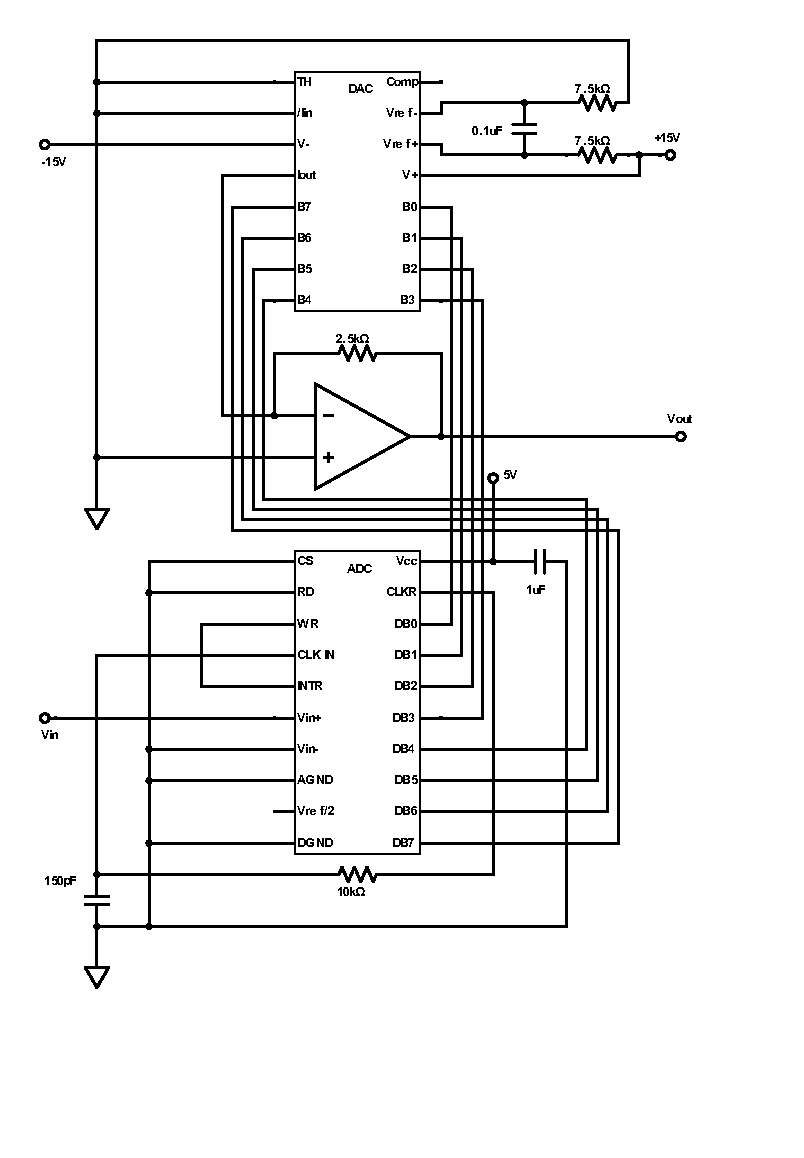
\includegraphics[width=0.49\textwidth]{image/ADC-DAC.pdf}
            \caption{Link the output of ADC to the input of DAC}
            \footnotetext{$V_\text{in}$ connect to SG}
            \label{fig:sine}
        \end{figure}
        \begin{figure}[t]
            \centering
            \subcaptionbox{Full 8 bit}[.49\linewidth][c]{%
                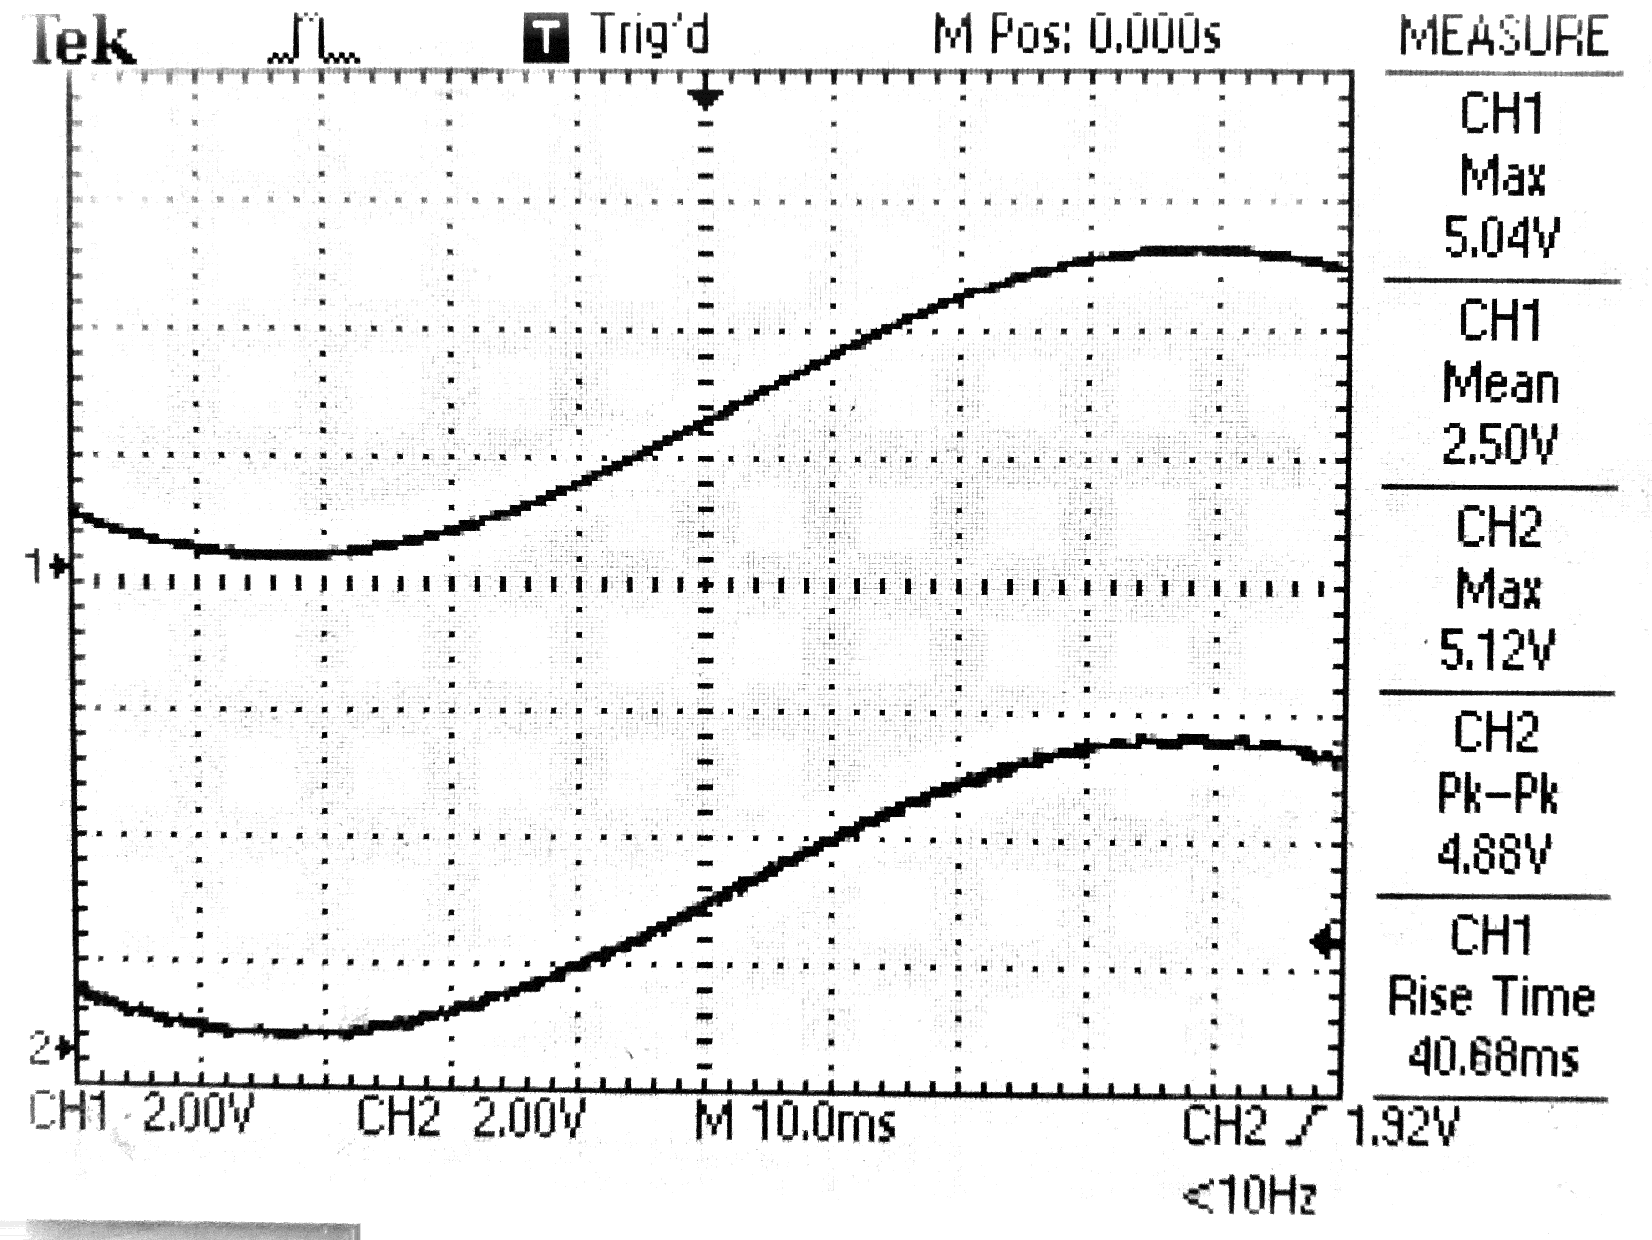
\includegraphics[width=.49\linewidth]{image/sine1.pdf}}\ 
            \subcaptionbox{Only 6 bit}[.49\linewidth][c]{%
                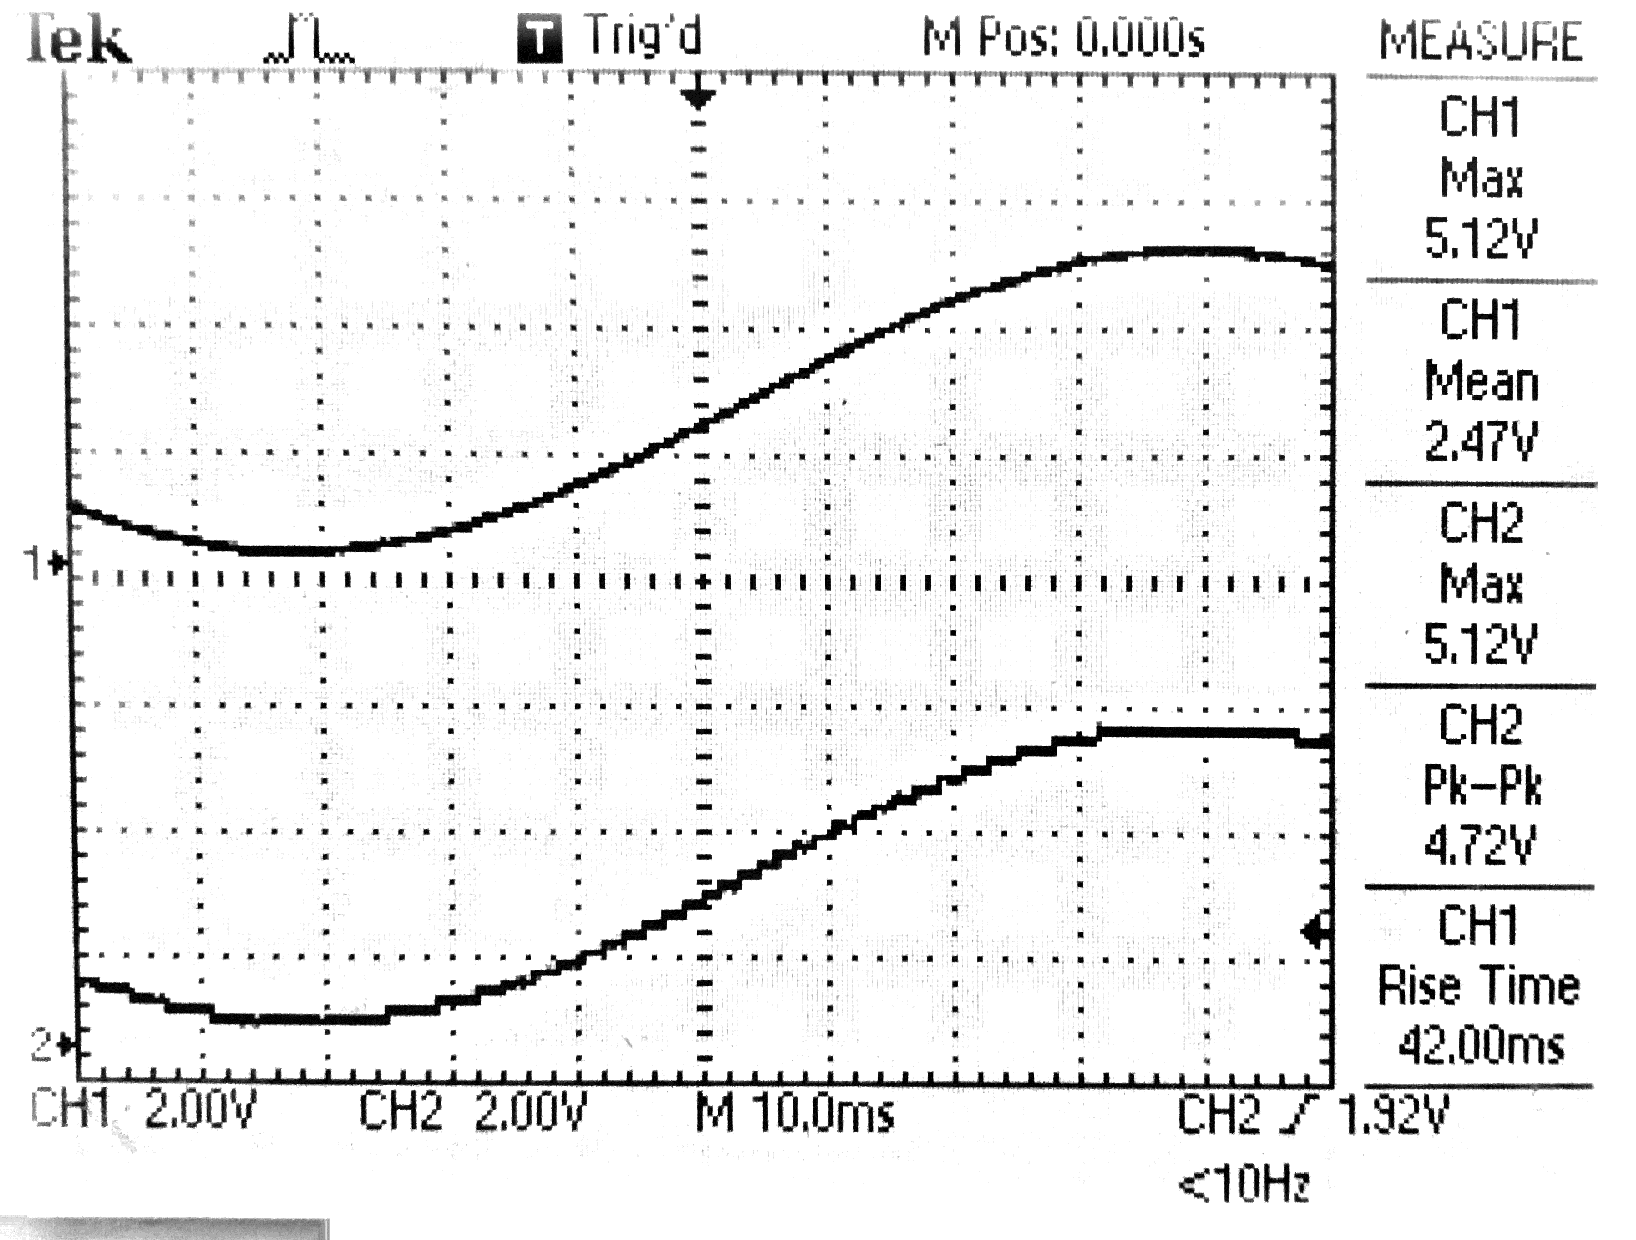
\includegraphics[width=.49\linewidth]{image/sine2.pdf}}\ 
            \caption{The result of digital sine wave}
            \label{fig:sinePlot}
        \end{figure}
        In this part, we connect the output of ADC to the input of DAC, as in Figure~\ref{fig:sine} and use a sine wave as a input of the ADC. The result is in Figure~\ref{fig:sinePlot}. We also disconnect the last least 2 bit to see a more digital result.
\section{Analysis}
    \subsection{ADC}
        The result of ADC is great. We see the linear fit is almost completely coincide with the data obtained. The small voltage on zero input might due to a background voltage, which cause a offset.
    \subsection{DAC}
        The result of DAC is also great. The input is same as the output as it should be.
    \subsection{Sine Wave}
        The result of the sine wave is good. The output match the input but with a small distortion. We see that for a smaller number of bit, the distortion incrence. We can add more bit to achieve a better result.
\section{Conclusion}
    The result of this lab is good. To reduced the jaggedness, we can use more bit.



\bibliography{cite}
\bibliographystyle{apsrev4-1}

    % \begin{figure}[h]
    %     \centering
    %     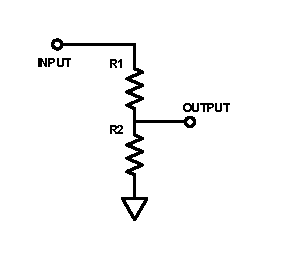
\includegraphics{images/plot2.pdf}
    %     \caption{A voltage divider}
    %     \label{fig:2}
    % \end{figure}

    % \begin{table}[h]
    % \begin{ruledtabular}
    % \begin{tabular}{cccc} 
    % Load[k$\Omega$] &  Output Voltage[V] & $R_\text{th}[\Omega]$ & Theoretical Voltage\\ \hline\hline
    % 50              & 0.680(1)           & 501(1)                & 0.682 \\ \hline
    % 500             & 3.75(1)            & 500(1)                & 3.75 \\ \hline
    % 5000            & 6.80(1)            & 514(1)                & 6.82 \\
    % \end{tabular}
    % \end{ruledtabular}
    % \caption{Load resistor and the output}
    % \label{table:8}
    % \end{table} 

% \begin{center}
%  \includegraphics[height=1.8in]{plot.pdf}
% \end{center} 

%\begin{center}
% \includegraphics[height=1.3in]{plot.pdf}
%\end{center}

% \blindtext \cite{article-minimal}

% \bibliographystyle{apsrev4-1} % Tell bibtex which bibliography style to use
% \bibliography{xampl} % Tell bibtex which .bib file to use (this one is some example file in TexLive's file tree)

\end{document}